\documentclass[11pt,a4paper]{article}
\usepackage[T1]{fontenc}
\usepackage[utf8]{inputenc}
\usepackage{lmodern}
\usepackage[margin=25mm]{geometry}
\usepackage{amsmath,amssymb,booktabs,tabularx,array,graphicx,microtype}
\usepackage[hidelinks]{hyperref}
\graphicspath{{../}{figures/}}
\setlength{\emergencystretch}{2em}
\newcolumntype{Y}{>{\raggedright\arraybackslash}X}
\newcommand{\KL}{D_{\mathrm{KL}}}
\newcommand{\ARL}{\mathrm{ARL}}
\newcommand{\repo}{\url{https://github.com/Rigur-Calypso/quantum-loss-change-detection}}
\title{Quantum-enhanced transmission-loss detection\\
\large Implementation, numerical comparisons and open questions}
\author{Bhagyesh Kamal}
\date{29 October 2026}
\begin{document}
\maketitle
\begin{abstract}
I implemented an independent Python study of Guha, John, Gong and Basu's
\emph{Quantum-enhanced quickest change detection of transmission loss}
(arXiv:2503.12276v2). The implementation covers coherent, squeezed,
entangled and single-photon observation models, sequential detectors and
false-alarm calibration. The analytical Figure~2 curves and the quoted
single-photon relative entropy are reproduced. Several published detection
delays and receiver comparisons remain unmatched. This report distinguishes
those discrepancies from successful mathematical checks, describes additional
validation studies and records the limits of the comparison. All quantum
models are simulated on a classical computer; no optical experiment is claimed.
\end{abstract}

\section{Question and scope}
The paper studies how to detect a sudden increase in optical transmission loss
while light pulses may also carry information~\cite{paper}. Its principal
proposal adds a small amount of squeezed light, independently or entangled
across pulse groups, to a much brighter coherent signal. A homodyne receiver
then measures the light and a sequential statistical test accumulates evidence
of a change. The favourable-regime improvement scale discussed in the paper is
$1/(1-\eta_1)$, which is ten for $\eta_1=0.9$; this is not a claim of a
tenfold improvement in every finite simulation. Increasing the entangled block
size at fixed $N_a$ requires stronger seed squeezing.

My aim was to implement these models, compare independently simulated results
with the paper and its public data~\cite{dataset}, and investigate the reliability
of the false-alarm comparison. I use \emph{implemented} for a method present in
working code, \emph{formula reproduction} for a recalculated mathematical curve,
and \emph{numerical agreement} for a stated comparison with published values.
These are different levels of evidence. Passing an internal test is not
evidence that every published result has been reproduced.

The source, figures and evidence manifest are available at \repo.
The saved simulation ensembles are distributed separately in the repository's
v0.1.0 release~\cite{code}. The public author data are attributed to Guha and
Basu, as recorded by Zenodo; the paper has four authors.

\section{Models and detector}
\subsection{Coherent and squeezed pulses}
Let $\eta_1$ and $\eta_2$ be the channel transmission before and after a change,
with $\eta_2<\eta_1$. The first changed pulse is indexed by $\nu$.
For a fair energy comparison, the coherent baseline has energy $N+N_a$,
whereas the quantum-augmented signal has coherent energy $N$ and augmentation
energy $N_a$ per pulse. The implemented receiver laws, following the paper, are
\begin{align}
X\mid j&\sim\mathcal N(\mu_j,v_j),\\
\mu_j^{\rm coh}&=\sqrt{\eta_j}\sqrt{N+N_a},
&v_j^{\rm coh}&=\tfrac14,\\
\mu_j^{\rm sq}&=\sqrt{\eta_j}\sqrt N,
&v_j^{\rm sq}&=\frac{\eta_j e^{-2r}+1-\eta_j}{4},
\qquad r=\operatorname{asinh}\sqrt{N_a}.
\end{align}
Here $v_j$ is a variance, not a standard deviation. Gaussian measurements are
the classical outcomes of the proposed quantum-optical experiment.

For arbitrary positive Gaussian variances the code evaluates
\begin{align}
\ell(x)&=\log\frac{p_2(x)}{p_1(x)}
=\frac12\log\frac{v_1}{v_2}
+\frac{(x-\mu_1)^2}{2v_1}-\frac{(x-\mu_2)^2}{2v_2},\\
\KL(P_2\Vert P_1)
&=\frac12\left[
\frac{v_2}{v_1}-1-\log\frac{v_2}{v_1}
+\frac{(\mu_2-\mu_1)^2}{v_1}\right].
\end{align}
This includes the change in noise variance under squeezing. Keeping only a
mean shift would implement a different detector. KL and likelihood scores
use natural logarithms and are measured in nats.

\subsection{Entangled pulse groups}
For $n$ pulses, the squeezed seed has energy $nN_a$, so its squeezing parameter
is $s=\operatorname{asinh}\sqrt{nN_a}$. With
$u=(1,\ldots,1)^\mathsf T/\sqrt n$, the homogeneous block model can be written as
\begin{equation}
m_j=\sqrt{\eta_j N}\,\mathbf 1,\qquad
K_j=\tfrac14 I+(v_j-\tfrac14)uu^\mathsf T,\qquad
v_j=\frac{1-\eta_j+\eta_j e^{-2s}}4.
\end{equation}
The collective measurement $u^\mathsf TX$ contains the homogeneous block
likelihood information. Its joint KL is divided by $n$ for a per-pulse
comparison. Full covariance sampling and an independent dense calculation
check this reduction.

The pulse-by-pulse detector uses conditional densities given earlier
measurements in the same block. A Page reset does not erase that physical
history. If the loss changes inside a block, the simulator retains a mixed-loss
covariance rather than generating two independent block fragments.
I do not claim that this correlated detector has the independent-observation
CUSUM optimality guarantee; the paper also distinguishes these cases.

\subsection{Page CUSUM and performance conventions}
For independent observations the Page recursion~\cite{page} is
\begin{equation}
W_0=0,\qquad W_t=\max\{0,W_{t-1}+\ell(X_t)\},\qquad
T=\inf\{t:W_t>h\}.
\end{equation}
The implementation uses the first strict threshold crossing, one-based pulse
indices and an earliest-prefix convention for tied change-point estimates.
An ordinary cumulative sum without reflection at zero is not this detector.

I distinguish the no-change average run length and the simulated delay:
\begin{equation}
\ARL=\mathbb E_\infty[T],\qquad
d_\nu=\mathbb E_\nu[T-\nu\mid T\geq\nu].
\end{equation}
An alarm on pulse $\nu$ therefore has delay zero. An earlier alarm is recorded
as a false alarm, not restarted or turned into a negative detection delay.
Right-censored runs are recorded explicitly; a finite-horizon restricted mean
is not presented as an unrestricted ARL or delay. The conditional mean $d_\nu$
is not Lorden's worst-case criterion~\cite{lorden}.

Thresholds are calibrated against false-alarm targets and frozen before
independent holdout checks. They are not fitted to the authors' delays.
For rare false alarms, regenerative cycle estimates, importance weights and
pooled moments supplement direct Monte Carlo. Monte Carlo uncertainty,
numerical mesh checks and weight diagnostics are reported as approximate
validation, not certified error bounds.

\section{Results that agree}
\begin{enumerate}
\item \textbf{Figure 2 formulas.} Coherent, independently squeezed and
$n=2,4,\ldots,256$ entangled per-pulse KL curves are recalculated for
$N=100$, $\eta_1=0.9$, $\eta_2=0.85$ and $N_a\in[0,5]$.
Closed forms and Gaussian calculations agree. This reproduces the analytical
construction; the inspected public dataset contains no numeric Figure~2 array for a
pointwise data comparison.
\item \textbf{Single-photon KL.} The implemented displaced Fock-1 homodyne law,
its CDF, an exact mixture sampler and numerical integration give
$0.2063404792$ nats, agreeing with the paper's rounded $0.2063$.
The calculated squeezing crossover is $1.812$~dB, close to its rounded
$1.83$~dB. This agreement does not resolve the delay comparison below.
\item \textbf{Large-ARL scaling.} Fourteen coherent/squeezed settings cover
target ARLs from $100$ to $10^8$ pulses. At high ARL, delay slopes normalized
by the expected $1/\KL$ slope are $1.000137694$ and $1.000084113$.
The largest deviation is about $0.014\%$. Finite-start offsets remain;
this is a numerical asymptotic check, not a new proof of the paper's Eq.~1.
\item \textbf{Optical statistics and weak probes.} Normalized Hadamard covariance
propagation agrees to below $2.8\times10^{-17}$ in the checked cases.
Seven approximate Figure~12 raster comparisons at $1$~dB have a maximum
relative difference of $1.67\%$. The latter is sparse pixel agreement, not
a complete reconstruction of that figure.
\end{enumerate}

\section{Differences from the published results}
Table~\ref{tab:gaps} lists unresolved comparisons. Relative differences use the author value as denominator. For Figure~3, absolute relative differences are averaged across energy points; Figure~7 reports the signed average by family. The numerical gaps are
descriptive: they do not by themselves establish an error in the paper.
Missing thresholds, raw event records or conventions can prevent a like-for-like
comparison even when the stated observation laws are implemented.

\begin{table}[htbp]
\centering\small
\caption{Published comparisons that remain unresolved. Figure numbers refer
to arXiv v2.}\label{tab:gaps}
\begin{tabularx}{\linewidth}{@{}p{20mm}YY@{}}
\toprule
Comparison & Independent result & Interpretation\\
\midrule
Figure 3 &
All eight author KL-ratio coordinates agree to numerical precision.
Mean absolute relative delay-ratio differences are $7.49\%$ without modulation
and $6.40\%$ with BPSK. &
Analytical agreement; incomplete latency agreement.\\
\addlinespace
Figure 4 &
At fixed seed squeezing, independent calculations give
$S_n=A/n+B$ with $A\geq0$, hence $S_1\geq S_2\geq S_4$.
The published inset places $n=2$ above $n=1$. &
The plotted ordering is not explained by the implemented fixed-seed model.\\
\addlinespace
Figure 5 &
Photon-number-resolving Kennedy KL values are $11.9$--$12.6$ times
four digitized published values. Independent integration and sampling agree. &
Neither on/off coarse-graining nor the checks performed resolve the discrepancy.\\
\addlinespace
Figure 7 &
Five detector families at nine energies: mean relative delay differences
are $13.65\%$, $25.89\%$, $34.39\%$, $30.60\%$, $28.63\%$
for coherent, squeezed, and entangled $n=2,4,8$. &
All family means are higher in our simulation; the 45 internal
ARL validation settings pass.\\
\addlinespace
Figure 11(b) &
Our single-photon conditional delay is $54.640\pm0.129$ pulses
(one standard error). The author array's signed mean is $48.034$. &
That array contains two negative values; event conventions are needed
before interpreting the means as the same quantity.\\
\bottomrule
\end{tabularx}
\end{table}

The public plotting files provide means and settings, but not the original Figure~3/7 thresholds, per-point standard errors or raw first-alarm records. The saved value $n=5000$ is treated as the observation horizon, not an inferred number of Monte Carlo trials.

The Figure~3/7 studies together have internal supporting ARL checks for
61 author-grid settings at a target of two million pulses. Passing those checks
does not prove equality with the authors' unpublished thresholds.

For Figure~5 the checked v2 parameters are $N=100$, $N_a=1$,
$\eta_{\rm tap}=0.9$, fractional amplitude error $0.01$ and phase variance
$0.01$, hence phase standard deviation $0.1$ rad. The energy-matched coherent
probe contains $101$ photons on average. A roughly ten-photon counterfactual
can approach the digitized curve, but it is a diagnostic hypothesis, not
a verified author parameter.

The Figure~11(b) study uses $30{,}000$ trials, $\nu=1000$ and a horizon of
$5000$ pulses. There are 17 early alarms, 29,983 survivors and no post-change
censoring. The author's raw latency vector contains $-844$ and $-129$.
Under the assumption that it contains complete first-alarm latencies, its
nonnegative re-summary is $50.181$ pulses. The remaining mean gap is
$4.459$ pulses, with bootstrap interval $[2.665,6.206]$ conditional on the
independence and missing-event assumptions used. This is not sufficient to
identify the reason for disagreement.

An ideal Kennedy null can have infinite KL because a click is impossible
under the ideal pre-change law. This does not mean zero waiting time at
finite signal energy: a changed pulse must still produce a click.

\section{Additional implementation studies}
These studies extend the computational investigation. I have not established
their research novelty through a broader literature review.
\begin{description}
\item[Rare false alarms.]
History-dependent mixture proposals, regenerative cycles, independent holdouts,
effective sample size and weight-concentration checks were used to examine
large ARLs. Follow-up validation supports all 25 points of one exploratory
grid; the historical failed records are retained.
\item[Incorrect initial-channel assumptions.]
When the detector assumes $\eta_1=0.9$, changing the true value from $0.899$
to $0.901$ changes the classical ARL from about $1.31$ to $3.01$ million pulses.
A small model mismatch can therefore undermine a nominally fair comparison.
\item[Conservative thresholds.]
Independent holdouts support adjusted approximate lower ARLs above two million
on 25 sampled detector/channel settings. The extra detection delay is
$3.61$--$4.39$ pulses for the classical detector and $1.12$--$2.33$ pulses for
the squeezed/entangled examples. This is sampled-grid evidence, not a guarantee
over a continuous parameter interval.
\item[Ideal dual-rail model.]
The Appendix~E.2 idea is developed into explicit arbitrary-qubit states, Kraus
loss maps and heralded survival. Uniform loss preserves a surviving state;
unequal rail loss can distort it. A herald is available after two time bins,
so pair counts and pulse counts are kept separate. Two holdouts support the
two-million-bin ARL target. No cavity dynamics, hardware implementation or
QKD-security proof is included.
\end{description}

\section{Reproducibility and remaining work}
The active package is \texttt{src/lossqcd}; original author files are preserved
under \texttt{data/authors}. Short module names describe the task:
\texttt{models}, \texttt{cusum}, \texttt{entangled}, \texttt{corr\_cusum},
\texttt{authors}, \texttt{photons}, \texttt{figures} and \texttt{report}.
Historical study paths and released archive names remain unchanged to preserve
provenance. The authors' plotting script is read as source material and is not
executed by the Python implementation.

The final verification checks 428 tests, 1,869 core evidence checks and
984 additional study checks. All 739 raw simulation array files and
572 metadata members are checked against the release manifest. These checks
recalculate saved evidence; they do not regenerate every trajectory. A fresh
execution of the introductory notebook separately checks the seeded lesson.
The dependency snapshot is recorded in \texttt{requirements.txt}; the source
and executed notebooks are \texttt{lesson.ipynb} and \texttt{example.ipynb}.

From the repository root, after installing the development dependencies:
\begin{verbatim}
python -m pytest -q
python -m lossqcd.lesson --output results/lesson_new
python -m lossqcd.evidence --scope all
python -m lossqcd.report --output results/review_new
python -m lossqcd.report --check results/review_new
\end{verbatim}
The evidence download is approximately 1.8~GiB for both raw archives.
Fresh output folders prevent accidental replacement of earlier records.
The README explains installation and the results report gives commands for
generating new ensembles.

The next useful step is to clarify the original Figure~3/7/11 thresholds and
event definitions, the Figure~4 fixed-seed calculation and the Figure~5
energy/receiver plotting calculation. The present evidence supports a
\textbf{partial numerical reproduction}. It does not establish full published
agreement, worst-case optimality for the correlated detector, a hardware
demonstration, a capacity-achieving communication code or the optimal
communication--detection tradeoff. The paper itself is a theoretical and
numerical study, so absent hardware does not explain our numerical gaps.

\clearpage
\appendix
\section{Selected computational results}
All images below are independent project outputs. Numbering in captions
identifies the paper comparison, not an exact reproduction claim.

\begin{figure}[htbp]
\centering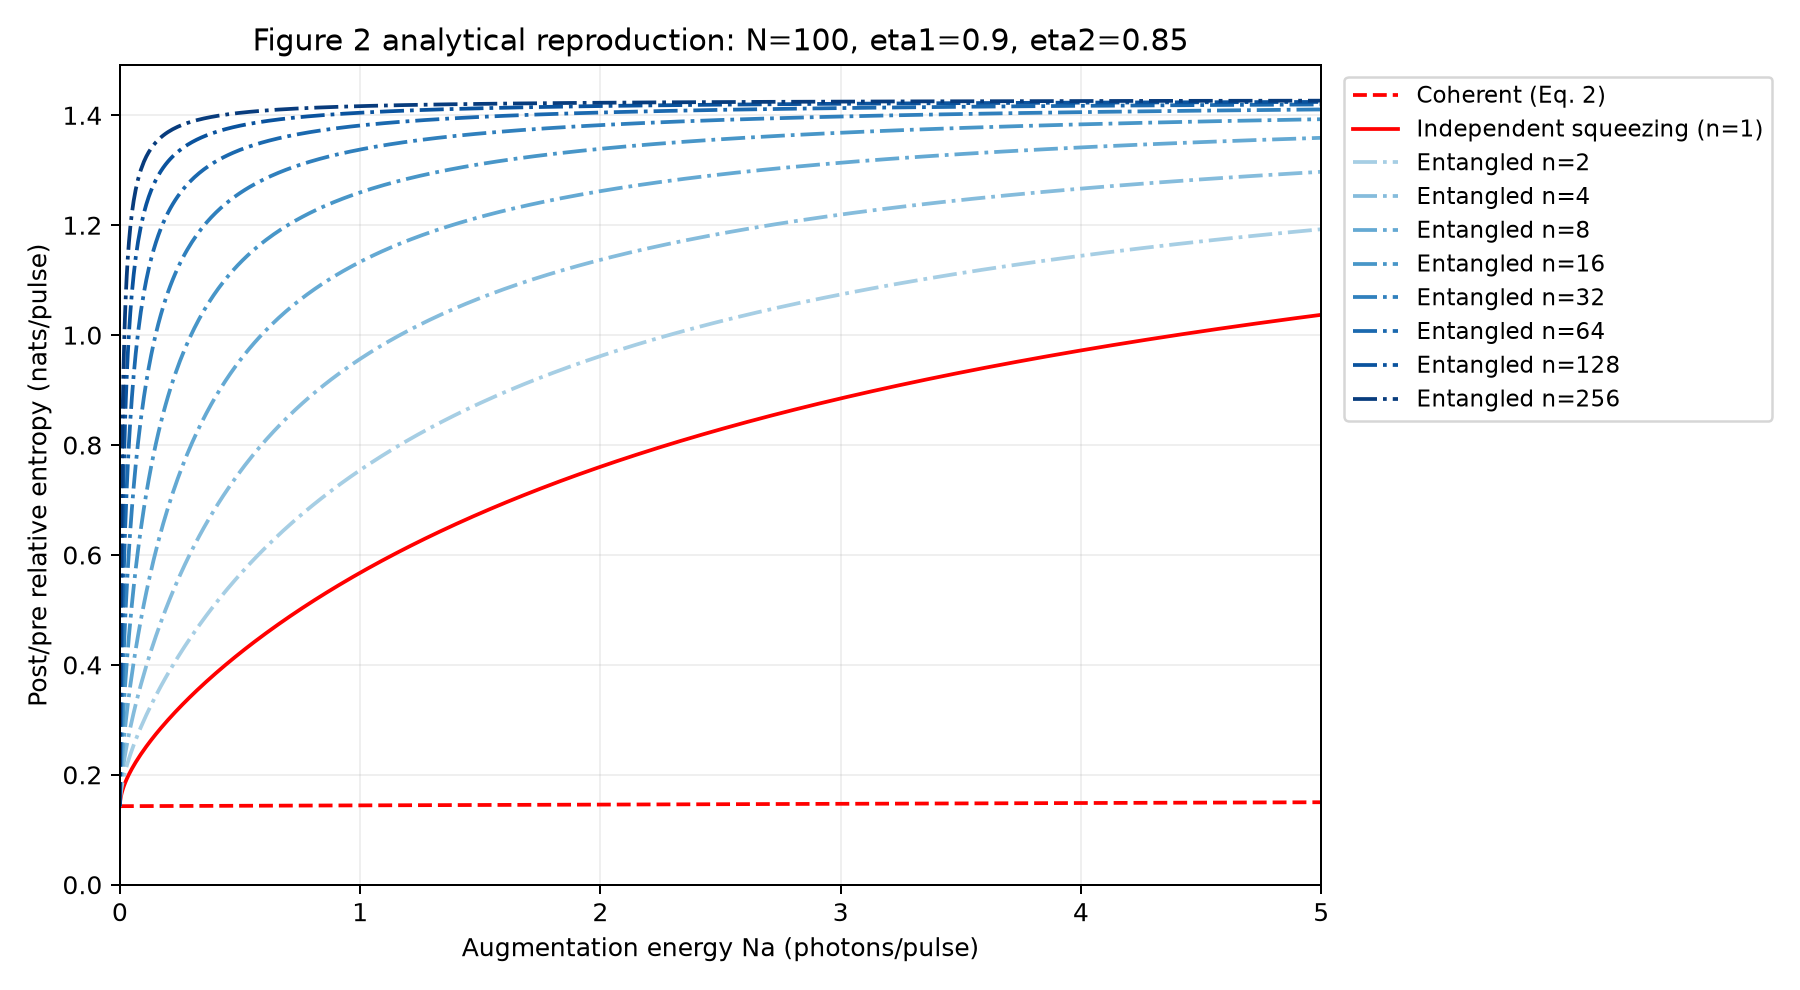
\includegraphics[width=.94\linewidth,height=.38\textheight,keepaspectratio]{figure2.png}
\caption{Figure 2 comparison: independently recalculated coherent, squeezed and
entangled KL curves. Formula reproduction; no original numeric array was available in the inspected dataset.}
\medskip
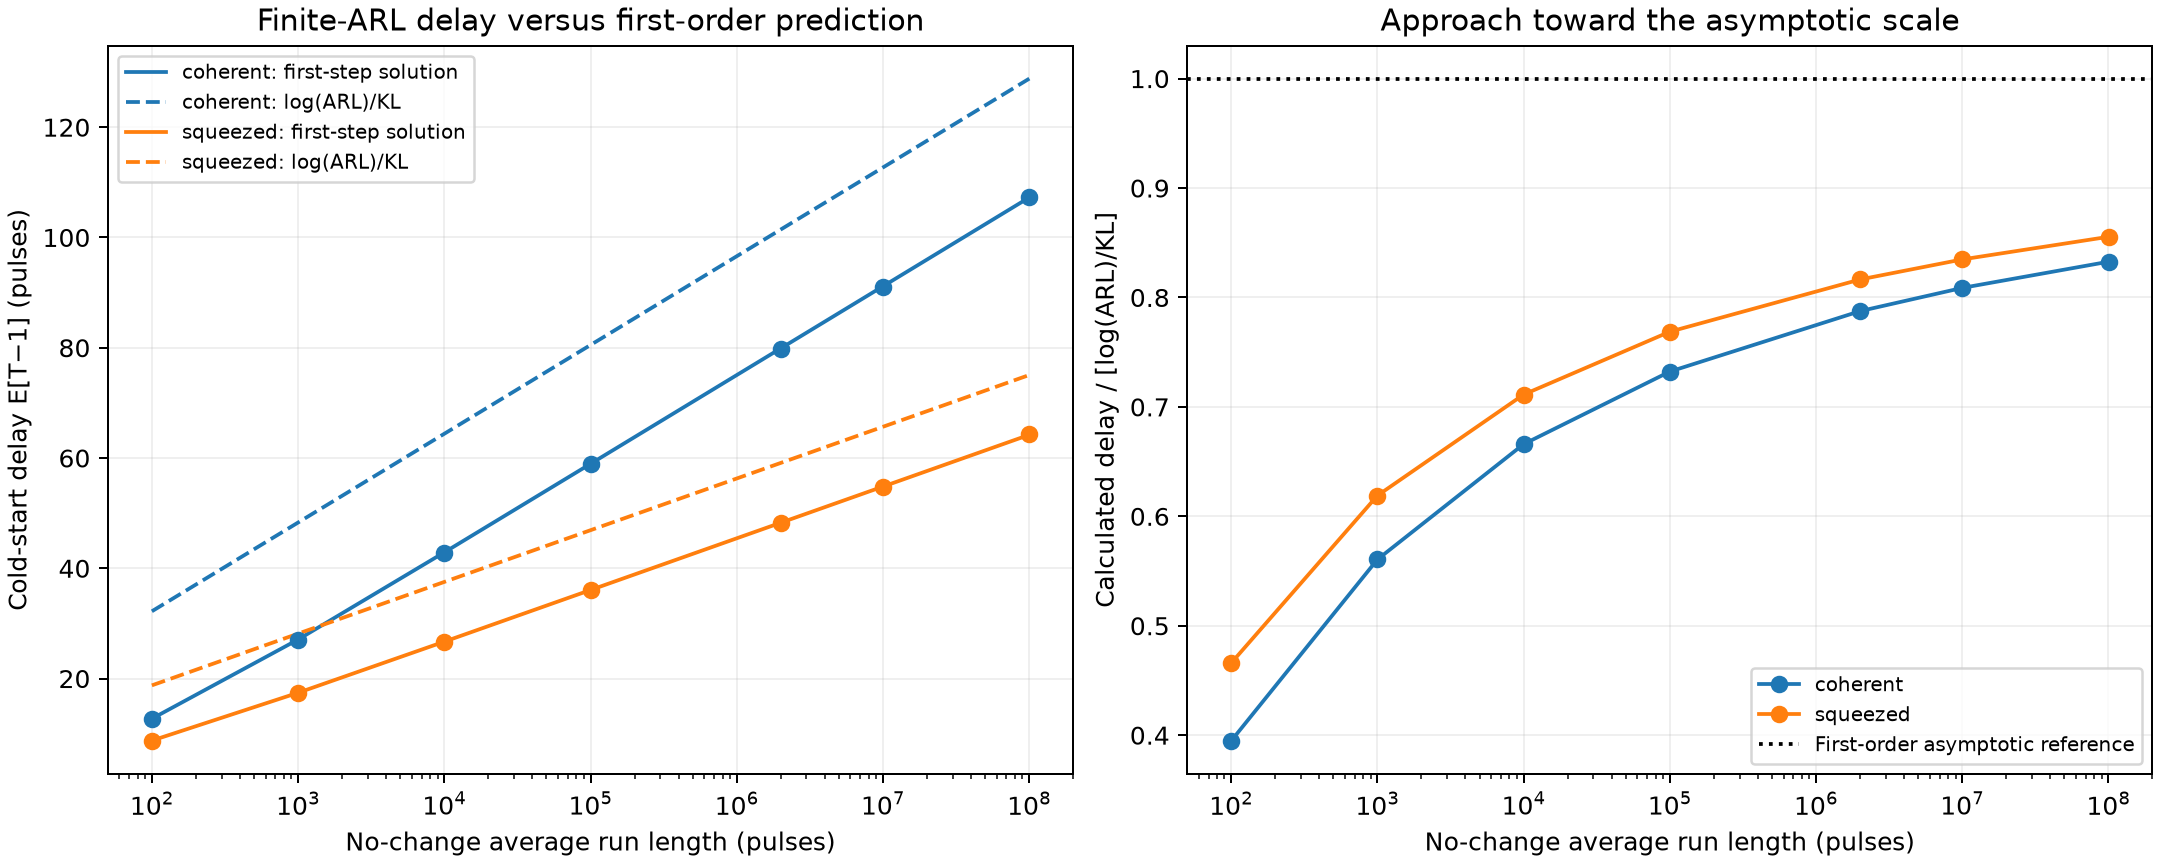
\includegraphics[width=.94\linewidth,height=.38\textheight,keepaspectratio]{scaling.png}
\caption{Additional finite-ARL scaling study. High-ARL slopes approach the
predicted inverse-KL scaling; finite-start offsets remain.}
\end{figure}

\begin{figure}[p]
\centering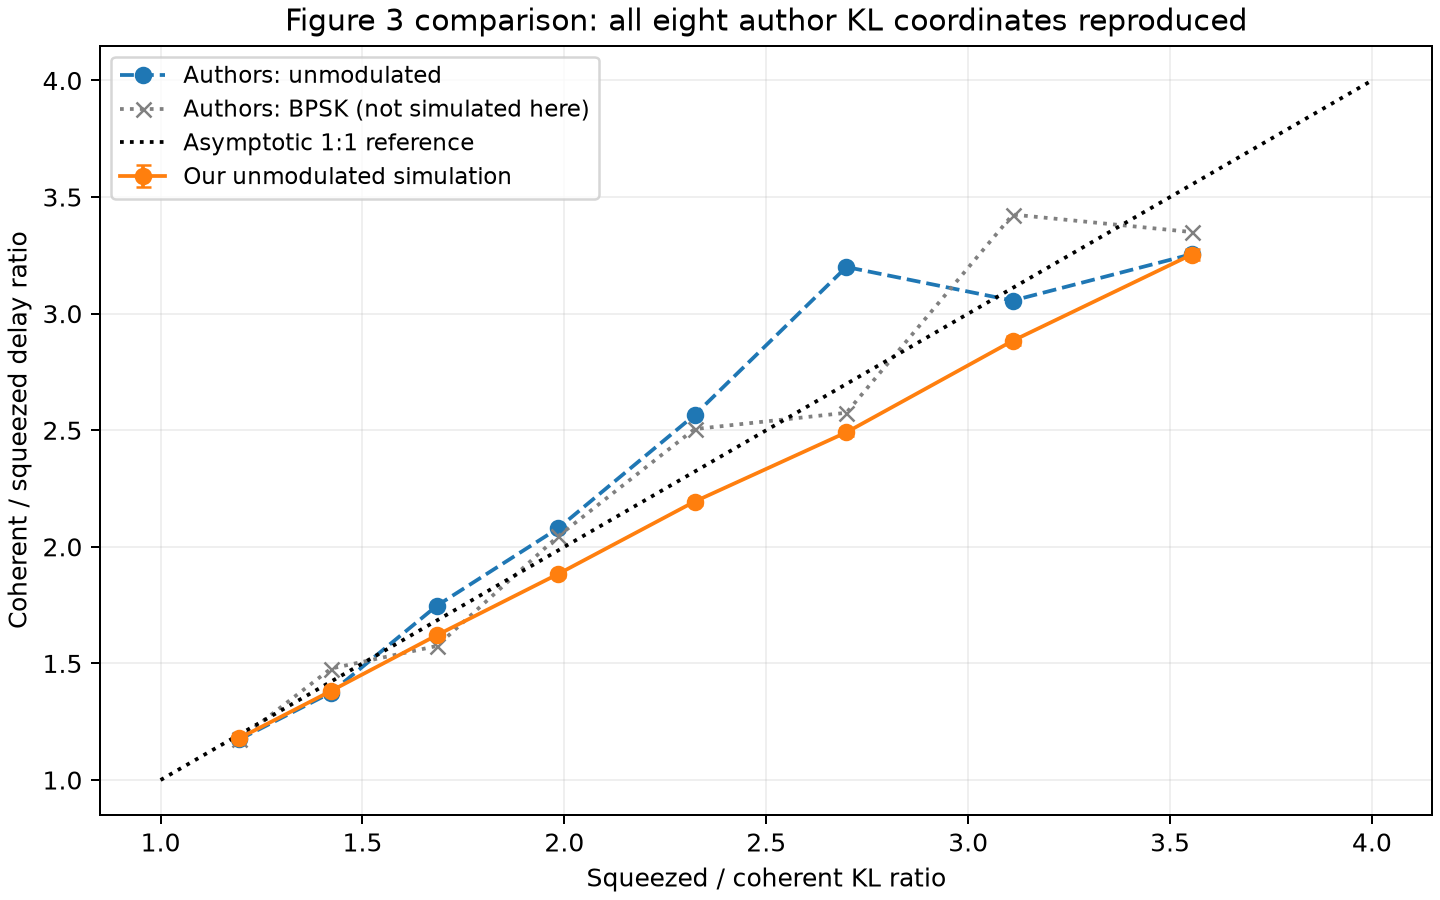
\includegraphics[width=.94\linewidth,height=.38\textheight,keepaspectratio]{figure3.png}
\caption{Figure 3 comparison: author and independent delay-improvement ratios.
KL coordinates agree; delay ratios remain different.}
\medskip
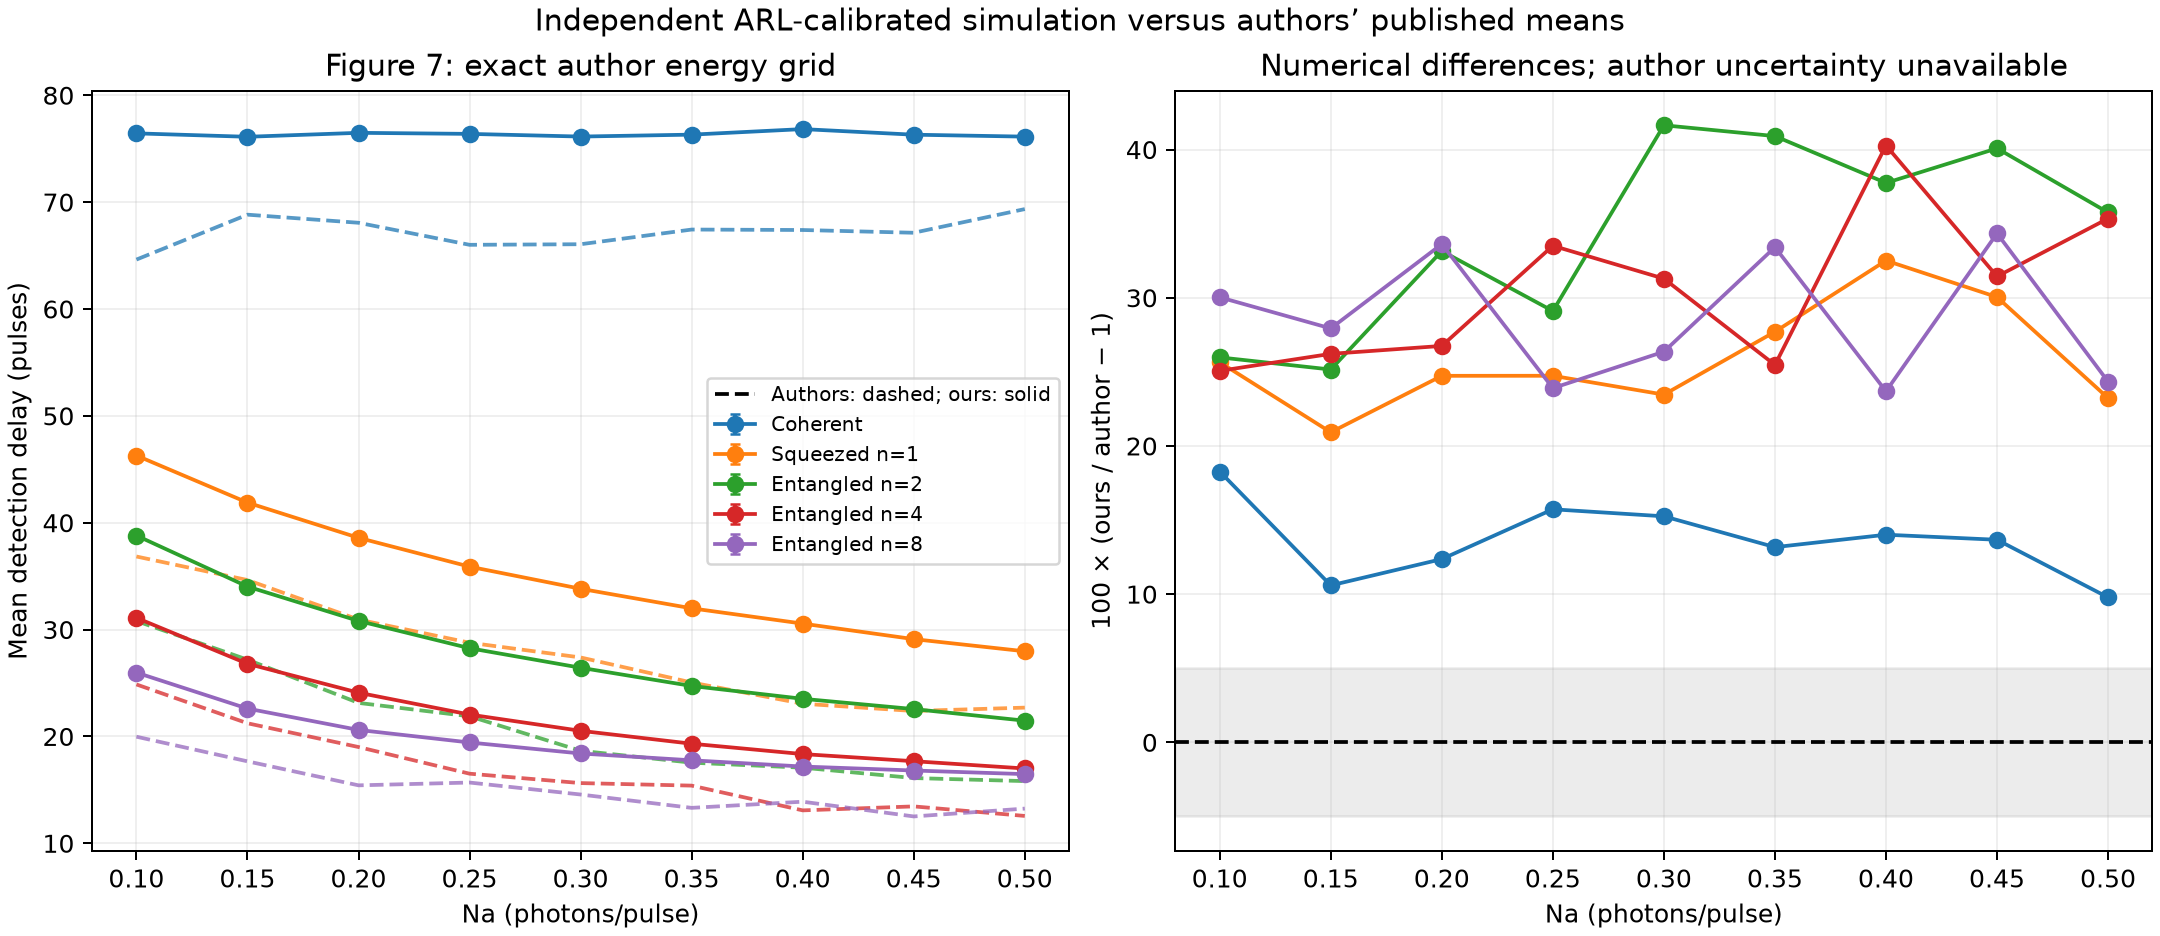
\includegraphics[width=.94\linewidth,height=.38\textheight,keepaspectratio]{figure7.png}
\caption{Figure 7 comparison: independently calibrated detectors and author
mean delays. Our family-average delays are higher.}
\end{figure}

\begin{figure}[p]
\centering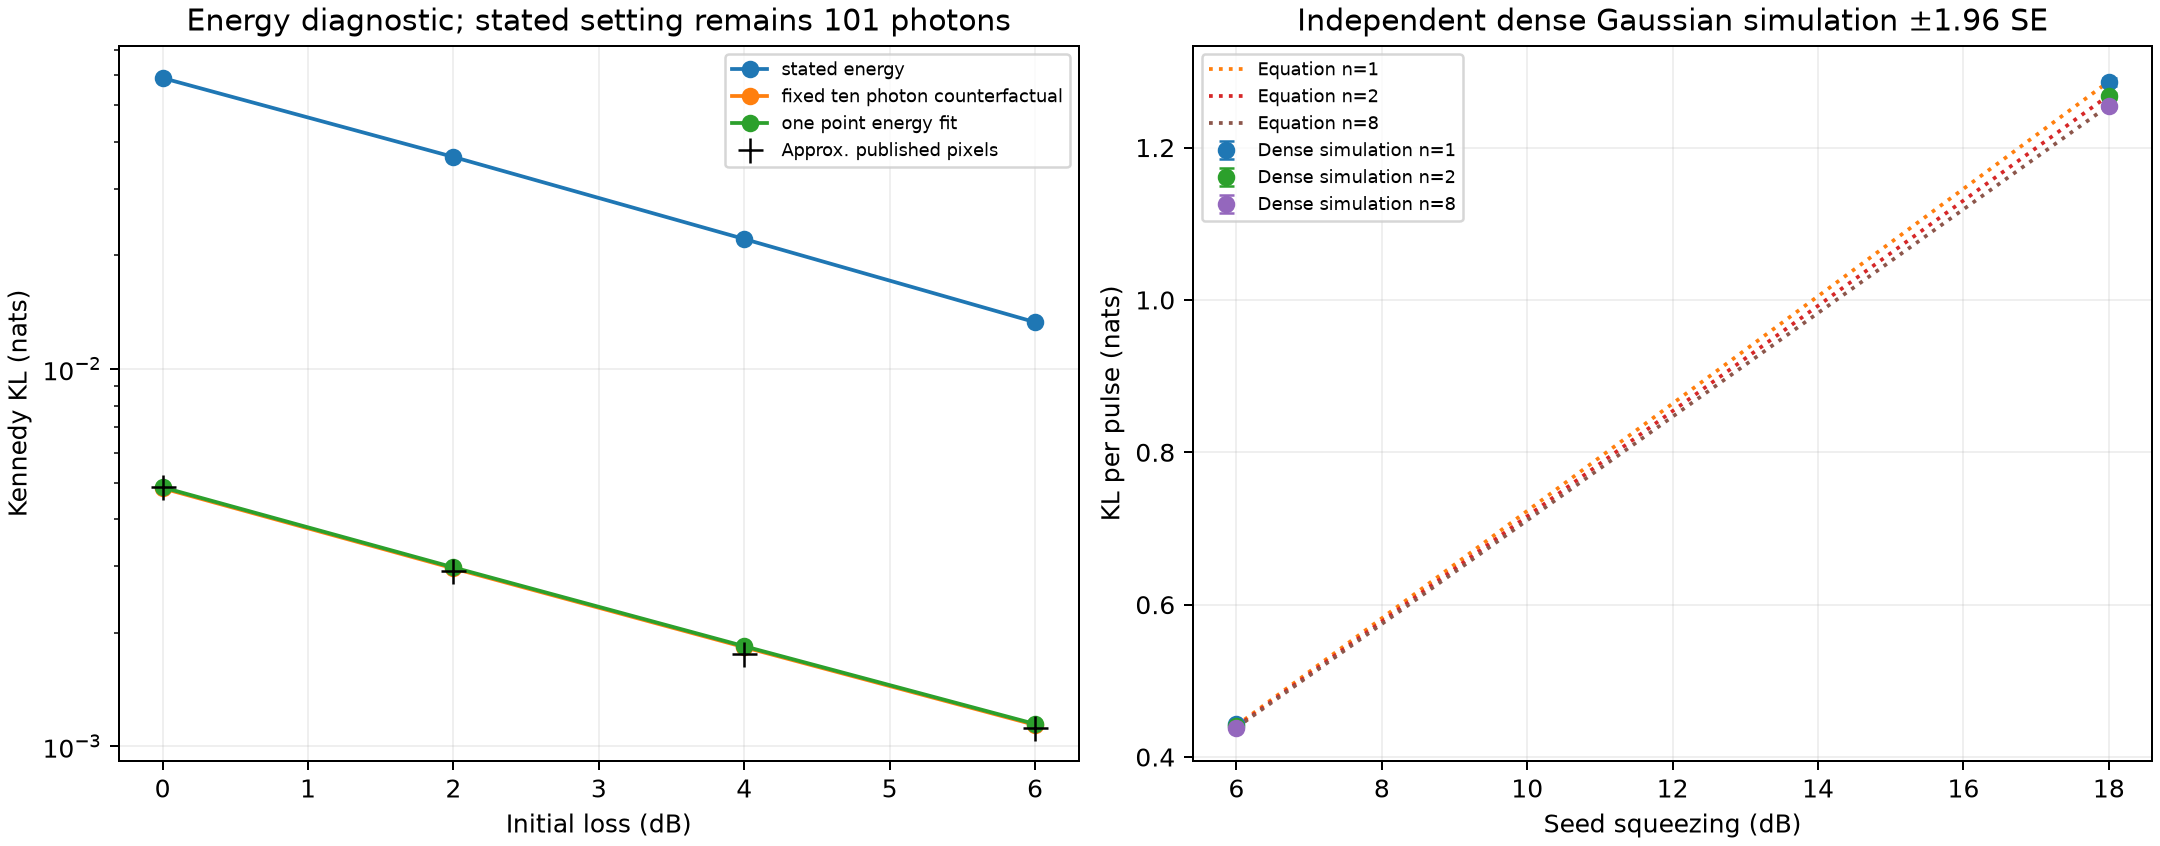
\includegraphics[width=.94\linewidth,height=.38\textheight,keepaspectratio]{figure5.png}
\caption{Independent checks of the fixed-seed Figure 4 and phase-noisy
Figure 5 equations. Diagnostic energy fits are not verified author settings.}
\medskip
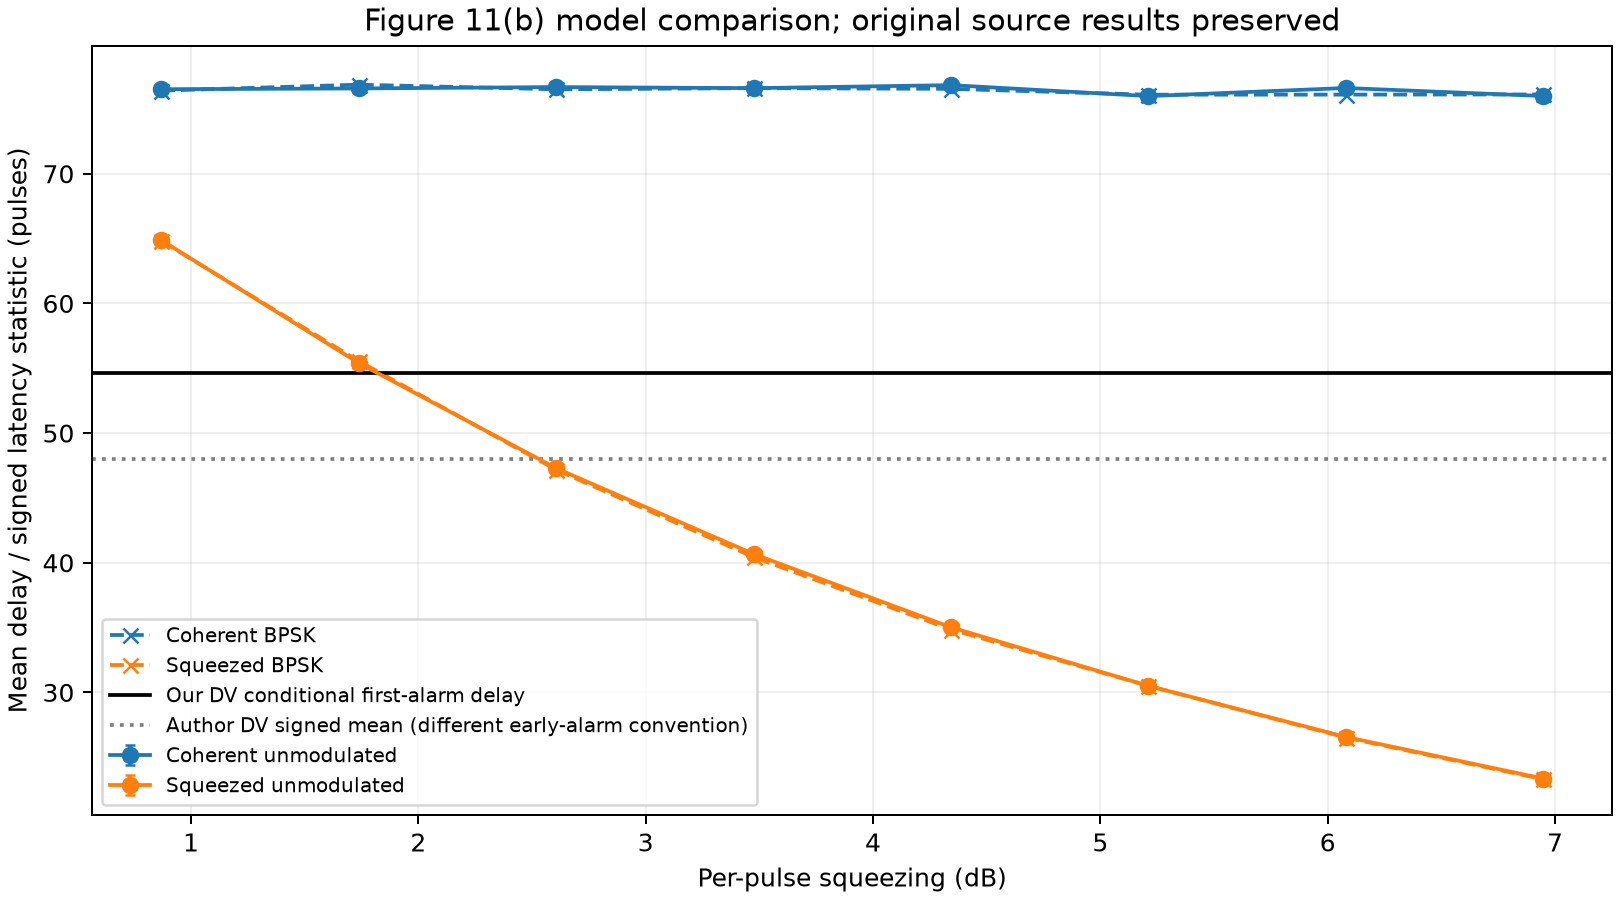
\includegraphics[width=.94\linewidth,height=.38\textheight,keepaspectratio]{figure11.png}
\caption{Single-photon and squeezed-light comparisons associated with Figure 11.
Entropy agreement and delay disagreement must be distinguished.}
\end{figure}

\begin{figure}[p]
\centering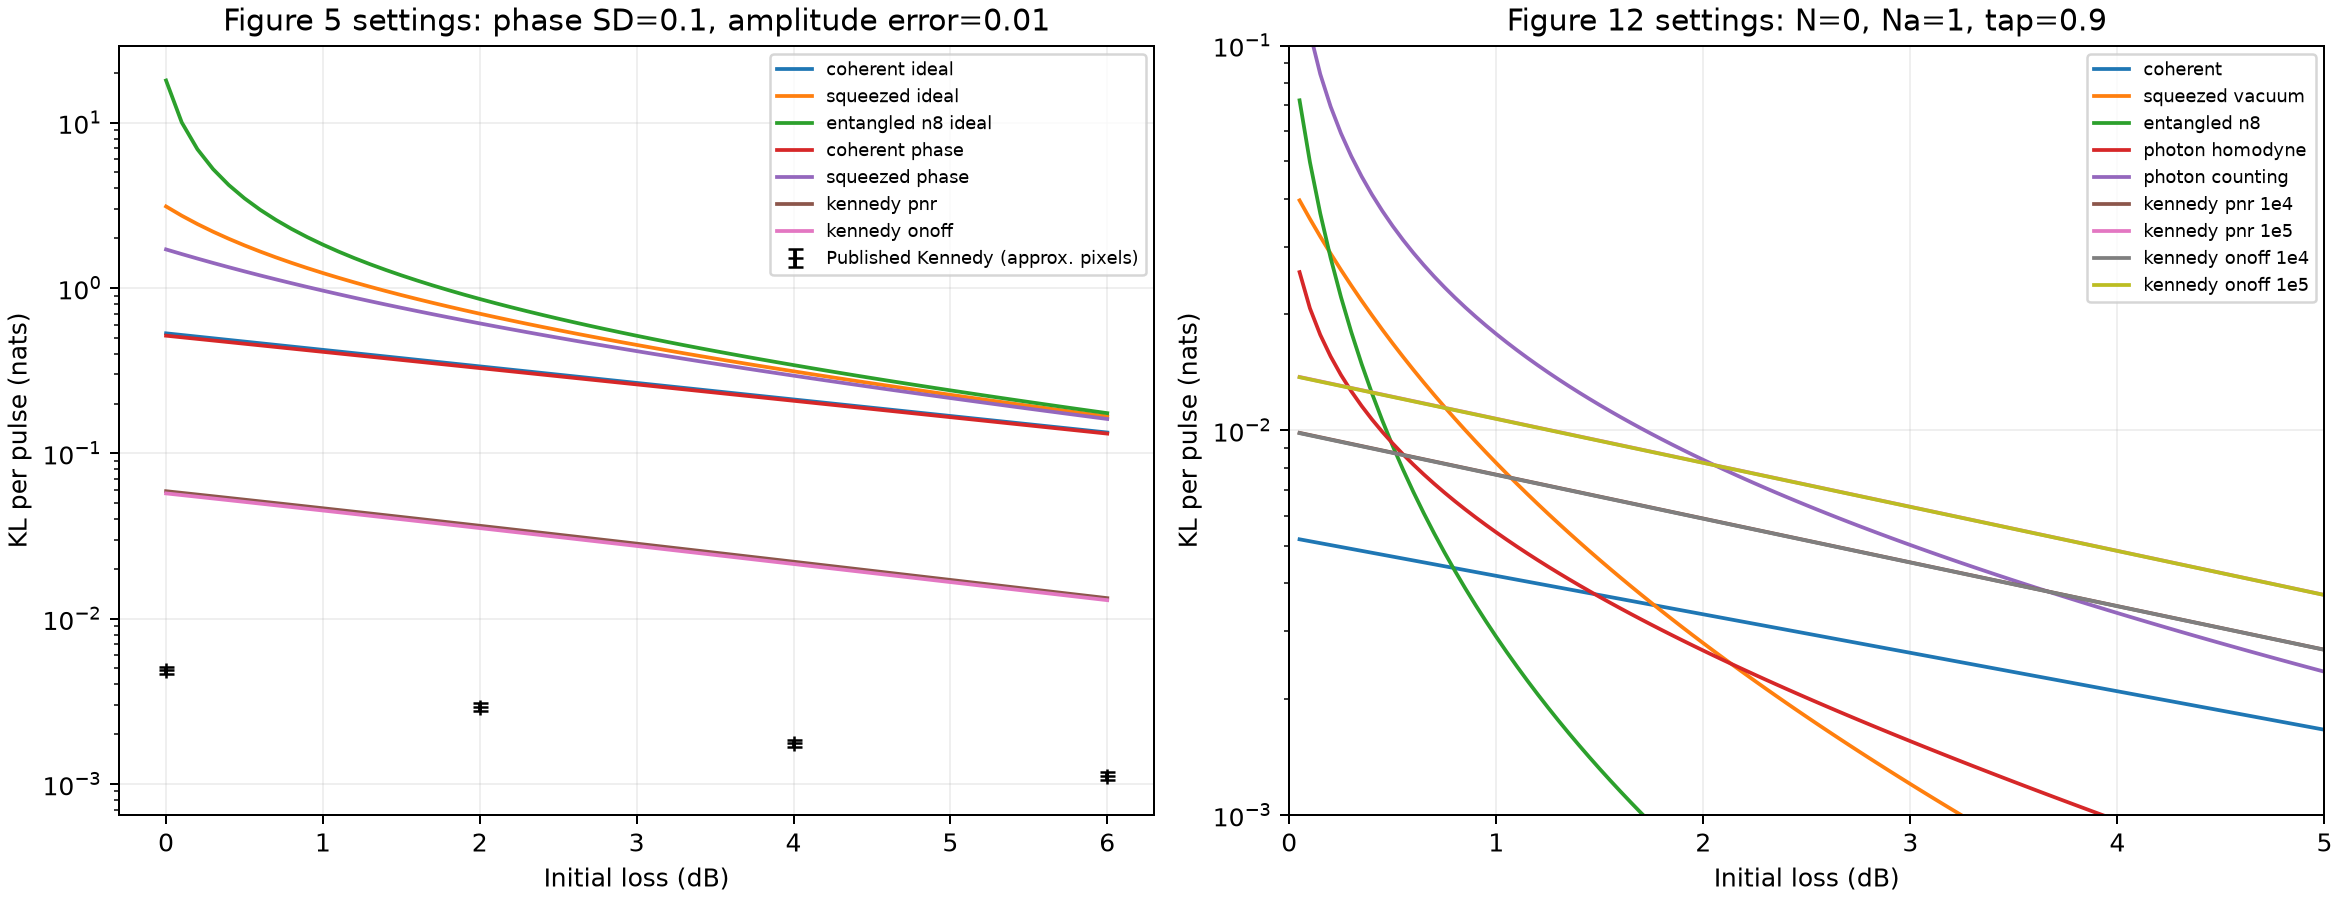
\includegraphics[width=.94\linewidth,height=.38\textheight,keepaspectratio]{figure12.png}
\caption{Weak-probe comparison associated with Figure 12. Only seven approximate
published raster values at 1 dB were checked; the full published curve is not validated.}
\medskip
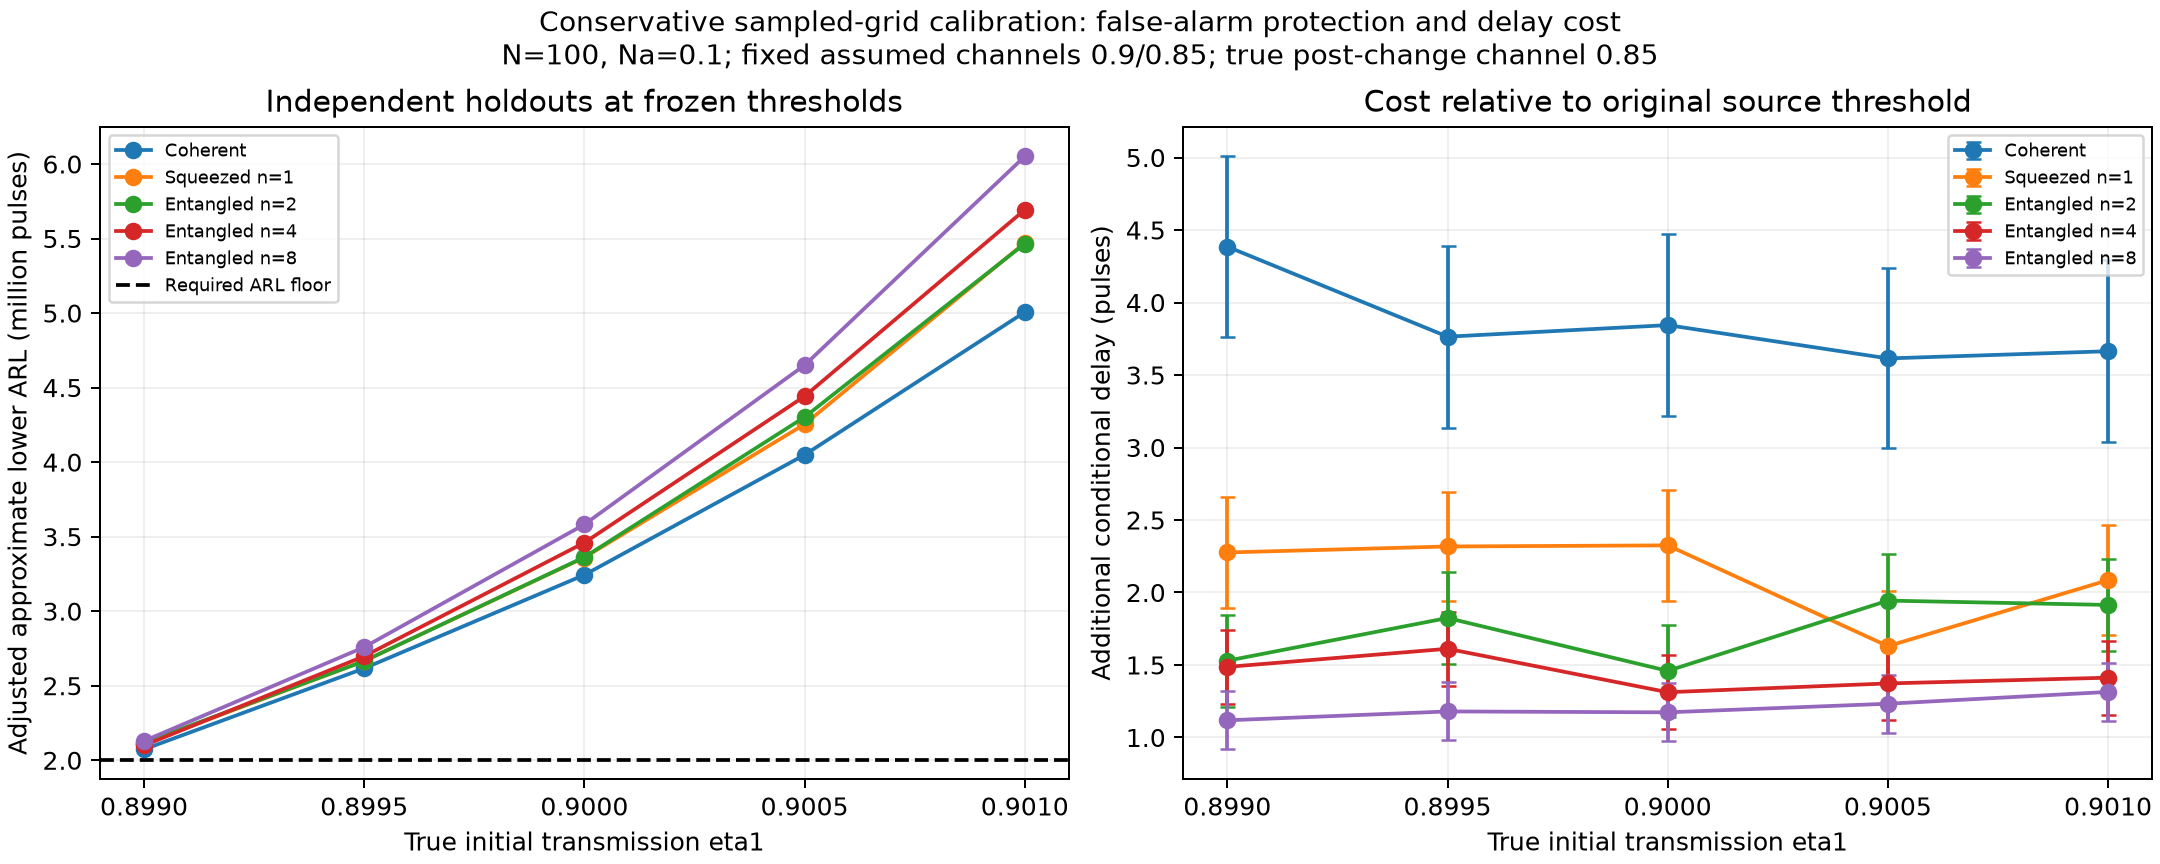
\includegraphics[width=.94\linewidth,height=.38\textheight,keepaspectratio]{robustness.png}
\caption{Additional sampled-grid study of conservative thresholds and
their detection-delay costs under initial-channel uncertainty.}
\end{figure}

\begin{figure}[p]
\centering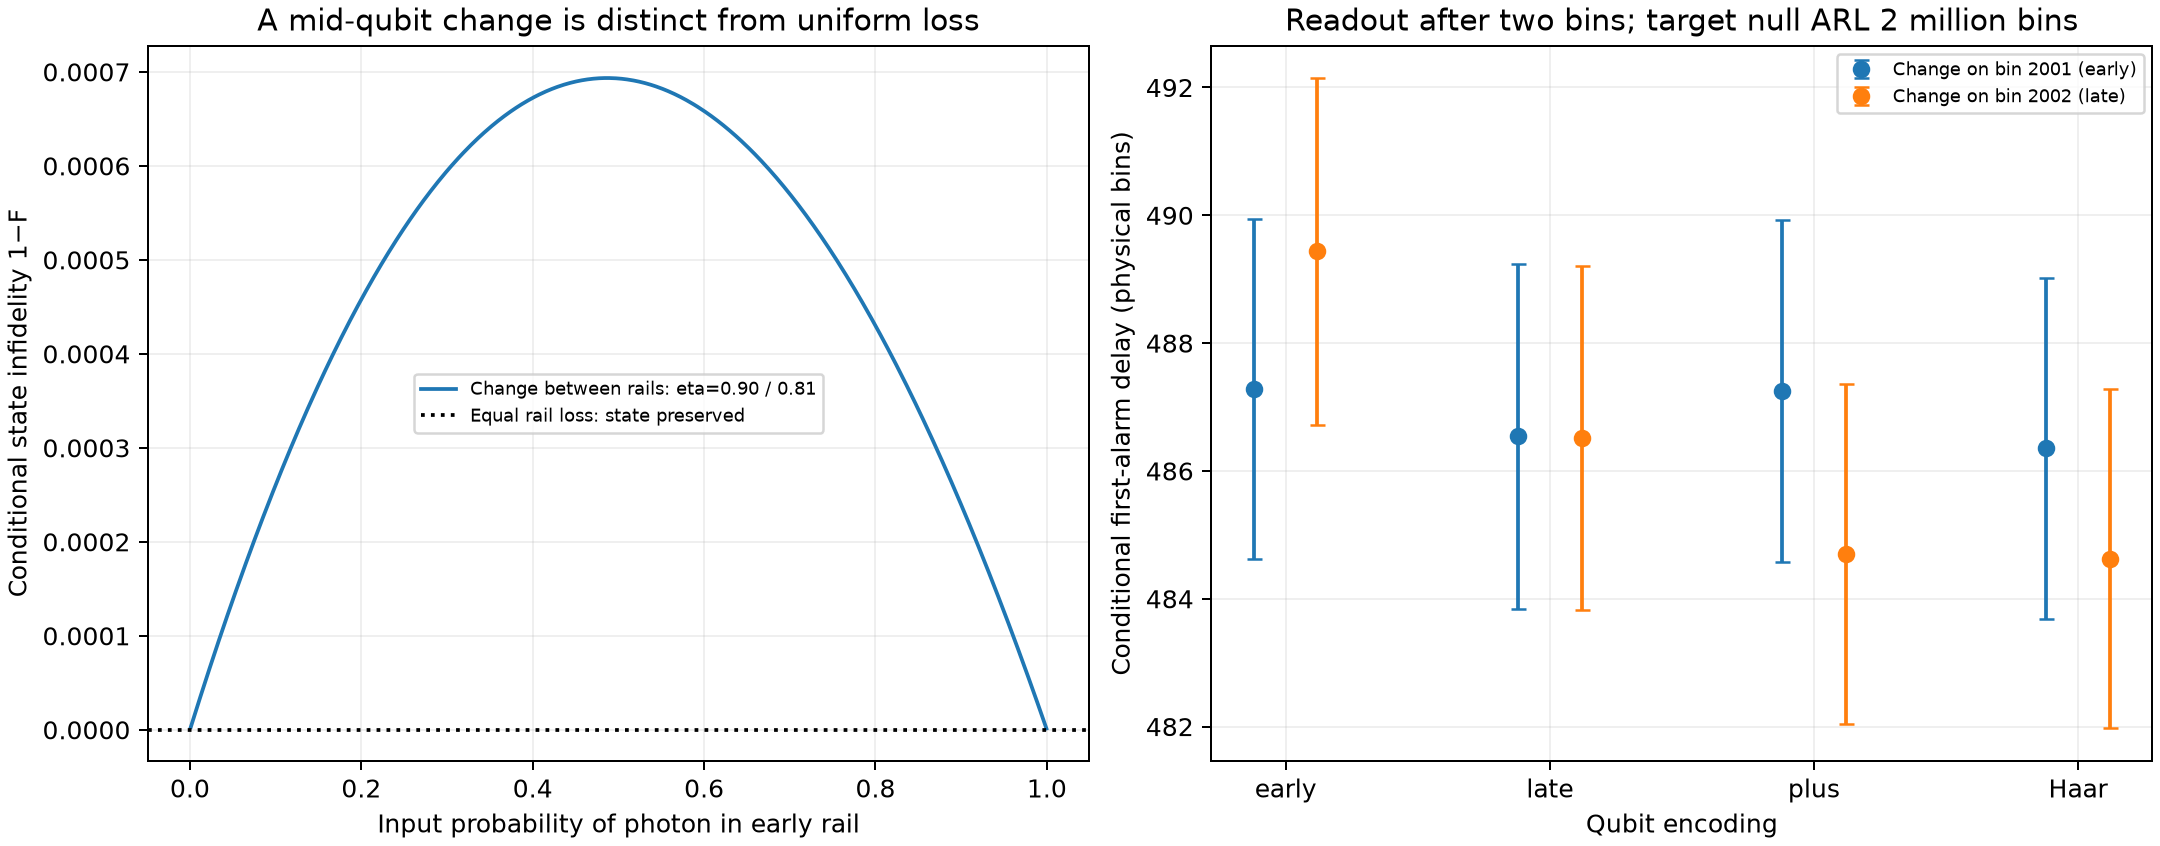
\includegraphics[width=.94\linewidth,height=.57\textheight,keepaspectratio]{dual_rail.png}
\caption{Ideal dual-rail channel extension based on Appendix E.2.
This is a mathematical channel simulation, without a cavity or QKD-security model.}
\end{figure}
\clearpage

\begin{thebibliography}{9}
\bibitem{paper}
S.~Guha, T.~C.~John, Z.~Gong and P.~Basu,
\emph{Quantum-enhanced quickest change detection of transmission loss},
arXiv:2503.12276v2, 1 November 2025.
\url{https://arxiv.org/html/2503.12276v2}.

\bibitem{dataset}
S.~Guha and P.~Basu,
\emph{Dataset accompanying PRL publication on quantum-enhanced quickest change
detection of transmission loss}, version v1, Zenodo, 2025.
\url{https://doi.org/10.5281/zenodo.17460928}.
Original data attribution and CC BY 4.0 terms are retained in the repository.

\bibitem{page}
E.~S.~Page,
\emph{On problems in which a change in a parameter occurs at an unknown point},
Biometrika \textbf{44}(1--2), 248--252 (1957).
Bibliographic details follow Ref.~11 of Guha et al.

\bibitem{lorden}
G.~Lorden,
\emph{Procedures for reacting to a change in distribution},
The Annals of Mathematical Statistics \textbf{42}(6), 1897--1908 (1971).
Bibliographic details follow Ref.~12 of Guha et al.

\bibitem{code}
B.~Kamal,
\emph{Quantum-loss change detection: implementation and simulation evidence},
repository and v0.1.0 raw-data release, accessed 29 October 2026.
\repo.
\url{https://github.com/Rigur-Calypso/quantum-loss-change-detection/releases/tag/v0.1.0}.
\end{thebibliography}
\end{document}
